\documentclass[aspectratio=169, 12pt]{beamer}
\usepackage{fontspec}
\setmainfont{Arial}

\usetheme{Madrid}
\usecolortheme{default}

\usepackage{graphicx}
\usepackage{amsmath}
\usepackage{listings}
\usepackage{booktabs}
\usepackage{xcolor}
\usepackage{tabularx}
\usepackage{caption}

% Set code listing style
\lstset{
    basicstyle=\ttfamily\scriptsize,
    breaklines=true,
    keywordstyle=\color{blue},
    stringstyle=\color{red},
    commentstyle=\color{green!60!black},
    showstringspaces=false,
    frame=single,
    backgroundcolor=\color{gray!10}
}

\title[ML - Chap 19]{Chương 19: Huấn luyện và Triển khai Mô hình TensorFlow Quy mô Lớn}
\author[Giảng viên]{Giảng viên}
\institute[Đại học Đông Á]{Đại học Đông Á}
\date{\today}

\begin{document}

% 1
\begin{frame}
    \titlepage
\end{frame}

% 2
\begin{frame}{Mục tiêu của Chương}
    \begin{itemize}
        \item Đưa mô hình ML vào môi trường thực tế (Production) với \textbf{TensorFlow Serving} và \textbf{Vertex AI}.
        \item Đưa AI lên Thiết bị di động (Mobile) và thiết bị nhúng với \textbf{TFLite}.
        \item Chạy AI trực tiếp trên trình duyệt bằng \textbf{TensorFlow.js}.
        \item Tối ưu hóa hiệu năng tính toán với \textbf{GPU / TPU}.
        \item Phân tán khối lượng huấn luyện khổng lồ trên hàng nghìn máy chủ với \textbf{Distribution Strategies API}.
    \end{itemize}
\end{frame}

% 3
\begin{frame}{Mục lục}
    \tableofcontents
\end{frame}

%==================================================================
\section{1. Phục vụ một mô hình TensorFlow (TF Serving)}
%==================================================================

% 4
\begin{frame}{1.1 Vòng đời dự án Machine Learning (MLOps)}
    \begin{itemize}
        \item Có được một mô hình học máy đạt độ chính xác cao mới chỉ là \textbf{bước khởi đầu}.
        \item Một kỹ sư ML thực thụ phải biết cách đưa mô hình đó ra phục vụ hàng triệu người dùng (Deployment).
        \item \textbf{MLOps (Machine Learning Operations)}: Tự động hóa quá trình huấn luyện, triển khai, theo dõi và cập nhật mô hình một cách mượt mà.
    \end{itemize}
\end{frame}

% 5
\begin{frame}{1.2 Những thách thức khi đưa AI vào Thực tế}
    \begin{itemize}
        \item \textbf{Khả năng mở rộng (Scalability):} Hệ thống phải chịu tải được hàng ngàn request mỗi giây mà không bị sập.
        \item \textbf{Độ trễ (Latency):} Người dùng yêu cầu nhận được dự đoán (VD: Dịch thuật, Nhận diện) ngay lập tức.
        \item \textbf{Quản lý phiên bản (Versioning):} Phải liên tục nạp mô hình mới (chính xác hơn) lên server mà không làm gián đoạn dịch vụ cũ (Zero Downtime).
    \end{itemize}
\end{frame}

% 6
\begin{frame}{1.3 Giới thiệu TensorFlow Serving}
    \begin{columns}
        \begin{column}{0.5\textwidth}
            \begin{itemize}
                \item \textbf{TensorFlow Serving (TFS)}: Công cụ bằng C++ hiệu năng cực cao của Google, chuyên dùng để chạy các mô hình ML trong Production.
                \item Thay vì dùng Flask hay Django (rất chậm vì dùng Python), TFS tối ưu hóa khả năng tận dụng GPU và CPU đa luồng.
            \end{itemize}
        \end{column}
        \begin{column}{0.5\textwidth}
            \centering
            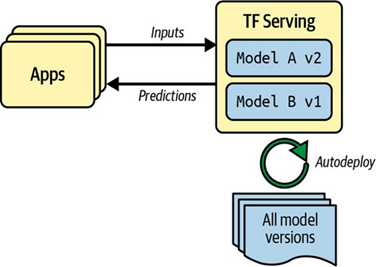
\includegraphics[width=\textwidth,height=0.65\textheight,keepaspectratio]{../machineLearningWeb/Figures/CH19/Hình_19-1.png}
            \vspace{0.2cm}
            \textit{Hình 19-1: Hệ sinh thái TensorFlow Extended (TFX) \& TF Serving}
        \end{column}
    \end{columns}
\end{frame}

% 7
\begin{frame}{1.4 Kiến trúc của TensorFlow Serving}
    \begin{itemize}
        \item TFS liên tục theo dõi một thư mục mô hình.
        \item Bất cứ khi nào bạn thả một thư mục phiên bản mới (VD: \texttt{v2}) vào, TFS sẽ tự động tải nó lên bộ nhớ.
        \item Request mới sẽ được chuyển hướng sang \texttt{v2}, trong khi các request cũ vẫn chạy trên \texttt{v1} cho đến khi xong hẳn, rồi \texttt{v1} mới bị xóa.
    \end{itemize}
\end{frame}

% 8
\begin{frame}[fragile]{1.5 Xuất mô hình (Exporting Model)}
    \begin{itemize}
        \item Để dùng được TFS, ta phải lưu mô hình dưới định dạng \textbf{SavedModel}.
        \item Thư mục SavedModel chứa: file \texttt{saved\_model.pb} (kiến trúc mạng) và thư mục \texttt{variables} (trọng số).
    \end{itemize}
\begin{lstlisting}[language=Python]
import tensorflow as tf

model = ... # Huan luyen mo hinh xong
model_version = "0001"
model_name = "my_mnist_model"
model_path = os.path.join(model_name, model_version)

# Luu thanh dinh dang SavedModel
tf.saved_model.save(model, model_path)
\end{lstlisting}
\end{frame}

% 9
\begin{frame}{1.6 REST API và gRPC}
    \begin{columns}
        \begin{column}{0.5\textwidth}
            \begin{itemize}
                \item TFS hỗ trợ 2 giao thức mạng:
                \item \textbf{REST API:} Dùng JSON qua HTTP. Dễ cấu hình, dễ debug, thích hợp cho Ứng dụng Web. (Chậm hơn vì phải parse JSON).
                \item \textbf{gRPC:} Giao thức nhị phân của Google. Cực kỳ nhanh, băng thông thấp. Phù hợp cho giao tiếp Server-to-Server.
            \end{itemize}
        \end{column}
        \begin{column}{0.5\textwidth}
            \centering
            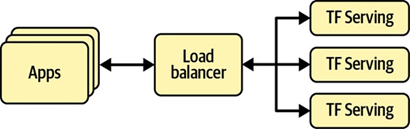
\includegraphics[width=\textwidth,height=0.65\textheight,keepaspectratio]{../machineLearningWeb/Figures/CH19/Hình_19-2.png}
            \vspace{0.2cm}
            \textit{Hình 19-2: REST vs gRPC trong giao tiếp Microservices}
        \end{column}
    \end{columns}
\end{frame}

% 10
\begin{frame}{1.7 Tạo dịch vụ Dự đoán trên Vertex AI (Google Cloud)}
    \begin{columns}
        \begin{column}{0.45\textwidth}
            \begin{itemize}
                \item Bạn không cần tự thuê Server và cài Docker TFS!
                \item \textbf{Vertex AI} là nền tảng quản lý MLOps toàn diện của Google Cloud.
                \item Bạn chỉ cần upload \texttt{SavedModel} lên Cloud Storage, nhấn Deploy, Google sẽ tự động tạo Endpoint (API) cho bạn.
            \end{itemize}
        \end{column}
        \begin{column}{0.55\textwidth}
            \centering
            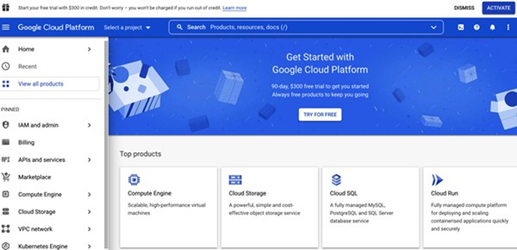
\includegraphics[width=\textwidth,height=0.65\textheight,keepaspectratio]{../machineLearningWeb/Figures/CH19/Hình_19-3.png}
            \vspace{0.2cm}
            \textit{Hình 19-3: Quy trình đưa Mô hình lên Vertex AI}
        \end{column}
    \end{columns}
\end{frame}

% 11
\begin{frame}[fragile]{1.8 Mã nguồn Triển khai trên Vertex AI}
\begin{lstlisting}[language=Python]
from google.cloud import aiplatform

# 1. Tai mo hinh tu Google Cloud Storage vao Vertex AI Model Registry
model = aiplatform.Model.upload(
    display_name="my_mnist_model",
    artifact_uri="gs://my-bucket/my_mnist_model/0001",
    serving_container_image_uri="us-docker.pkg.dev/vertex-ai/prediction/tf2-cpu.2-8:latest"
)

# 2. Trien khai mo hinh len mot Endpoint
endpoint = model.deploy(
    machine_type="n1-standard-4",
    min_replica_count=1,
    max_replica_count=5 # Tu dong scale len 5 may chu neu tai cao
)
\end{lstlisting}
\end{frame}

% 12
\begin{frame}{1.9 Dự đoán Hàng loạt (Batch Predictions)}
    \begin{itemize}
        \item Endpoint ở trên dùng cho \textbf{Online Prediction} (Cần trả lời ngay lập tức từng ảnh một).
        \item Nếu ta có 1 triệu bức ảnh trong Cloud Storage cần phân loại (không vội), ta sẽ dùng \textbf{Batch Prediction}.
        \item Vertex AI sẽ tự động mượn hàng trăm máy tính, chạy đồng loạt mô hình, ghi kết quả ra file, rồi tắt máy tính để tiết kiệm tiền.
    \end{itemize}
\end{frame}

% 13
\begin{frame}{1.10 Tóm tắt: Tự quản lý vs Dùng Cloud (Vertex AI)}
    \begin{itemize}
        \item \textbf{Tự cài TF Serving (On-premise):} Rẻ hơn, kiểm soát hoàn toàn dữ liệu. Nhưng tốn công bảo trì, cấu hình Load Balancer, Kubernetes phức tạp.
        \item \textbf{Dùng Vertex AI:} Tốn tiền dịch vụ Cloud, nhưng Google tự lo phần Scaling, Load Balancing, và Bảo mật. Giúp kỹ sư ML tập trung vào Mô hình.
    \end{itemize}
\end{frame}


%==================================================================
\section{2. Triển khai AI lên Thiết bị Di động \& Web}
%==================================================================

% 14
\begin{frame}{2.1 Edge AI - Trí tuệ Nhân tạo tại biên}
    \begin{columns}
        \begin{column}{0.5\textwidth}
            \begin{itemize}
                \item Tại sao phải đưa AI xuống chạy trực tiếp trên Điện thoại / Smartwatch?
                \item \textbf{Độ trễ thấp nhất:} Không cần gửi ảnh lên server.
                \item \textbf{Hoạt động Offline:} Vẫn dùng được khi rớt mạng.
                \item \textbf{Bảo mật:} Dữ liệu cá nhân (Khuôn mặt, Giọng nói) không bao giờ rời khỏi thiết bị.
            \end{itemize}
        \end{column}
        \begin{column}{0.5\textwidth}
            \centering
            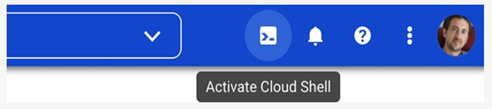
\includegraphics[width=\textwidth,height=0.65\textheight,keepaspectratio]{../machineLearningWeb/Figures/CH19/Hình_19-4.png}
            \vspace{0.2cm}
            \textit{Hình 19-4: Ứng dụng Edge AI trong đời sống}
        \end{column}
    \end{columns}
\end{frame}

% 15
\begin{frame}{2.2 Giới thiệu TensorFlow Lite (TFLite)}
    \begin{itemize}
        \item TFLite là một phiên bản "thu nhỏ" của TensorFlow, được thiết kế đặc biệt cho Điện thoại (Android, iOS) và Vi điều khiển (Arduino, ESP32).
        \item Dung lượng file thư viện TFLite chỉ tốn vài Trăm Kilobyte!
        \item Nó không có các hàm huấn luyện mạng (Train), chỉ chứa các hàm chạy dự đoán (Inference).
    \end{itemize}
\end{frame}

% 16
\begin{frame}{2.3 Quy trình chuyển đổi TFLite}
    \begin{columns}
        \begin{column}{0.4\textwidth}
            \begin{itemize}
                \item \textbf{Bước 1:} Train mô hình TF bình thường bằng Python.
                \item \textbf{Bước 2:} Dùng TFLite Converter để nén mô hình thành file \texttt{.tflite}.
                \item \textbf{Bước 3:} Nạp file \texttt{.tflite} vào app Android bằng Java/Kotlin và chạy Interpreter.
            \end{itemize}
        \end{column}
        \begin{column}{0.6\textwidth}
            \centering
            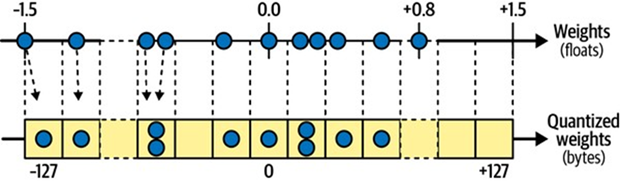
\includegraphics[width=\textwidth,height=0.65\textheight,keepaspectratio]{../machineLearningWeb/Figures/CH19/Hình_19-5.png}
            \vspace{0.2cm}
            \textit{Hình 19-5: Luồng công việc TFLite: Train, Convert, Deploy}
        \end{column}
    \end{columns}
\end{frame}

% 17
\begin{frame}{2.4 Tối ưu hóa: Lượng tử hóa (Quantization)}
    \begin{itemize}
        \item Trọng số nơ-ron mặc định lưu dưới dạng số thực 32-bit (Float32). Rất nặng!
        \item Lượng tử hóa (Quantization) chuyển trọng số thành số nguyên 8-bit (Int8).
        \item Lợi ích: \textbf{Giảm 4 lần dung lượng} mô hình. Tốc độ tính toán nhanh hơn.
        \item Cái giá: Giảm độ chính xác một chút xíu (khoảng 1-2\%).
    \end{itemize}
\end{frame}

% 18
\begin{frame}{2.5 Tối ưu hóa: Cắt tỉa mạng (Pruning)}
    \begin{columns}
        \begin{column}{0.5\textwidth}
            \begin{itemize}
                \item \textbf{Pruning:} Quá trình tìm và cắt đứt các kết nối (trọng số) có giá trị gần bằng 0 trong mạng nơ-ron.
                \item Mạng trở nên thưa thớt (Sparse). File nén \texttt{.zip} cực kỳ nhỏ bé.
                \item \textbf{Clustering:} Gom nhóm các trọng số giống nhau lại dùng chung 1 giá trị.
            \end{itemize}
        \end{column}
        \begin{column}{0.5\textwidth}
            \centering
            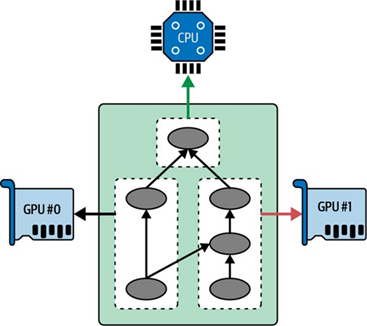
\includegraphics[width=\textwidth,height=0.6\textheight,keepaspectratio]{../machineLearningWeb/Figures/CH19/Hình_19-6.png}
            \vspace{0.2cm}
            \textit{Hình 19-6: Kỹ thuật cắt tỉa làm mỏng mạng nơ-ron (Pruning)}
        \end{column}
    \end{columns}
\end{frame}

% 19
\begin{frame}{2.6 Delegate: Khai thác phần cứng Mobile}
    \begin{itemize}
        \item Chạy AI trên CPU điện thoại sẽ làm nóng máy và tốn pin nhanh.
        \item TFLite hỗ trợ các \textbf{Delegate} để chuyển tính toán sang GPU điện thoại hoặc NPU (Neural Processing Unit).
        \item Ví dụ: Android Neural Networks API (NNAPI) hoặc Apple Core ML.
    \end{itemize}
\end{frame}

% 20
\begin{frame}{2.7 TensorFlow.js (TF.js)}
    \begin{columns}
        \begin{column}{0.4\textwidth}
            \begin{itemize}
                \item Đưa AI trực tiếp lên Trình duyệt Web (Chrome, Firefox)!
                \item Viết hoàn toàn bằng JavaScript/TypeScript.
                \item Khách truy cập web không cần cài đặt bất cứ thư viện nào, AI tự chạy phía Client!
            \end{itemize}
        \end{column}
        \begin{column}{0.6\textwidth}
            \centering
            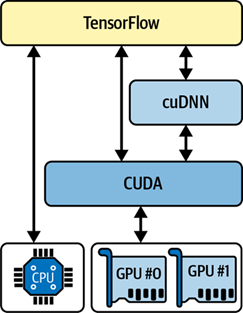
\includegraphics[width=\textwidth,height=0.65\textheight,keepaspectratio]{../machineLearningWeb/Figures/CH19/Hình_19-7.png}
            \vspace{0.2cm}
            \textit{Hình 19-7: Hệ sinh thái TensorFlow.js trên Browser và Node.js}
        \end{column}
    \end{columns}
\end{frame}

% 21
\begin{frame}{2.8 Đặc điểm nổi bật của TF.js}
    \begin{itemize}
        \item \textbf{Tận dụng WebGL / WebGPU:} TF.js tự động chuyển các phép nhân ma trận thành mã shader để chạy trên Card Đồ Họa của người dùng duyệt web.
        \item Tốc độ có thể đạt gần bằng chạy native (C++).
        \item Rất tuyệt vời cho các demo tương tác AI (ví dụ: Google Teachable Machine).
    \end{itemize}
\end{frame}

% 22
\begin{frame}[fragile]{2.9 Chuyển đổi mô hình cho Web}
    \begin{itemize}
        \item Để chạy được trên JS, ta phải chuyển \texttt{SavedModel} sang định dạng Web (\texttt{model.json} và file shard nhị phân).
    \end{itemize}
\begin{lstlisting}[language=bash]
# Cai dat tfjs converter
pip install tensorflowjs

# Lenh chuyen doi
tensorflowjs_converter \
    --input_format=keras \
    my_model.h5 \
    my_tfjs_model_folder
\end{lstlisting}
\end{frame}


%==================================================================
\section{3. Tăng tốc bằng GPU/TPU và Phân tán Tính Toán}
%==================================================================

% 23
\begin{frame}{3.1 Nhu cầu Phần cứng Chuyên dụng}
    \begin{itemize}
        \item Huấn luyện mô hình LLM (như GPT-4) hay CNN hàng tỷ tham số tốn cực nhiều phép nhân ma trận liên tiếp.
        \item CPU mất hàng năm trời để hoàn thành. Ta bắt buộc phải dùng \textbf{Phần cứng gia tốc (Accelerators)} như GPU hoặc TPU.
    \end{itemize}
\end{frame}

% 24
\begin{frame}{3.2 CPU so với GPU và TPU}
    \begin{columns}
        \begin{column}{0.45\textwidth}
            \begin{itemize}
                \item \textbf{CPU (Central Processing Unit):} Một vị giáo sư thông thái. Xử lý cực tốt logic phức tạp, nhưng chỉ có vài nhân (cores).
                \item \textbf{GPU (Graphics Processing Unit):} Hàng ngàn học sinh tiểu học. Chỉ biết làm toán cộng nhân đơn giản, nhưng làm đồng thời. Rất hợp cho Ma trận.
                \item \textbf{TPU (Tensor Processing Unit):} Chip do chính Google làm riêng cho phép nhân Ma trận.
            \end{itemize}
        \end{column}
        \begin{column}{0.55\textwidth}
            \centering
            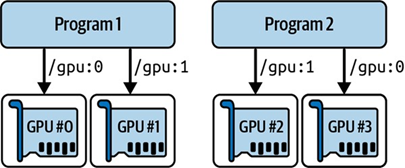
\includegraphics[width=\textwidth,height=0.65\textheight,keepaspectratio]{../machineLearningWeb/Figures/CH19/Hình_19-8.png}
            \vspace{0.2cm}
            \textit{Hình 19-8: CPU (ít ALU phức tạp) vs GPU (hàng ngàn ALU đơn giản)}
        \end{column}
    \end{columns}
\end{frame}

% 25
\begin{frame}{3.3 Làm sao có GPU để huấn luyện?}
    \begin{itemize}
        \item \textbf{Mua máy tính riêng (Local):} Đầu tư Card NVIDIA (RTX 4090). Cần cài CUDA Toolkit và cuDNN. Mất nhiều thời gian bảo trì.
        \item \textbf{Thuê Cloud VM:} AWS EC2 P3/P4, Google Cloud Compute. Chi phí tính theo giờ.
        \item \textbf{Google Colab / Kaggle:} Nền tảng Notebook trực tuyến cung cấp GPU/TPU miễn phí cho sinh viên và cá nhân. Tốt nhất để học!
    \end{itemize}
\end{frame}

% 26
\begin{frame}{3.4 Quản lý RAM GPU trong TensorFlow}
    \begin{columns}
        \begin{column}{0.45\textwidth}
            \begin{itemize}
                \item Theo mặc định, khi vừa bật lên, TensorFlow sẽ \textbf{chiếm toàn bộ VRAM} của GPU để tránh phân mảnh bộ nhớ.
                \item Nếu bạn muốn chạy 2 mô hình cùng lúc, mô hình 2 sẽ báo lỗi "Out of Memory" (OOM).
                \item Giải pháp: Bật tính năng \texttt{memory\_growth} (chỉ cấp phát bộ nhớ khi cần).
            \end{itemize}
        \end{column}
        \begin{column}{0.55\textwidth}
            \centering
            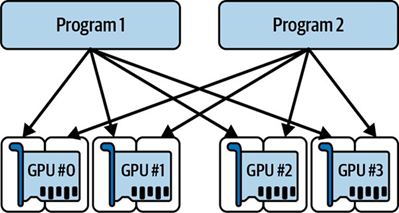
\includegraphics[width=\textwidth,height=0.65\textheight,keepaspectratio]{../machineLearningWeb/Figures/CH19/Hình_19-9.png}
            \vspace{0.2cm}
            \textit{Hình 19-9: Vấn đề tràn RAM GPU và cách khắc phục}
        \end{column}
    \end{columns}
\end{frame}

% 27
\begin{frame}[fragile]{3.5 Bật chế độ Memory Growth (Code)}
\begin{lstlisting}[language=Python]
import tensorflow as tf

physical_devices = tf.config.list_physical_devices('GPU')
if physical_devices:
    try:
        # Bat che do "can den dau cap den do"
        for gpu in physical_devices:
            tf.config.experimental.set_memory_growth(gpu, True)
    except RuntimeError as e:
        print(e)
\end{lstlisting}
\end{frame}

% 28
\begin{frame}{3.6 Huấn luyện trên Nhiều thiết bị (Multi-Device)}
    \begin{itemize}
        \item Khi 1 Card GPU (VD: VRAM 24GB) không chứa nổi Batch Size lớn, ta phải ghép 2, 4 hoặc 8 Card GPU lại trên cùng một bo mạch chủ (Multi-GPU).
        \item Nếu 8 Card vẫn không đủ, ta ghép 100 máy chủ lại với nhau (Mỗi máy có 8 Card) thông qua mạng tốc độ cao (Multi-Worker).
        \item Đây là cách mà siêu máy tính huấn luyện ChatGPT (Hàng chục ngàn GPU A100).
    \end{itemize}
\end{frame}

% 29
\begin{frame}{3.7 Cách TensorFlow chia tải: Placement}
    \begin{columns}
        \begin{column}{0.5\textwidth}
            \begin{itemize}
                \item TensorFlow biểu diễn mọi tính toán bằng \textbf{Đồ thị (Graph)}.
                \item Một thuật toán tên là *Placer* sẽ quyết định nút nào (Node) chạy trên CPU, nút nào chạy trên GPU 0, GPU 1.
                \item Ta có thể cưỡng ép thủ công: \texttt{with tf.device('/GPU:1'):}
            \end{itemize}
        \end{column}
        \begin{column}{0.5\textwidth}
            \centering
            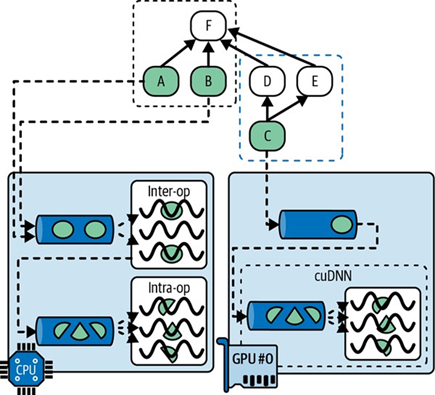
\includegraphics[width=\textwidth,height=0.6\textheight,keepaspectratio]{../machineLearningWeb/Figures/CH19/Hình_19-10.png}
            \vspace{0.2cm}
            \textit{Hình 19-10: Đồ thị tính toán phân bổ trên các thiết bị}
        \end{column}
    \end{columns}
\end{frame}

% 30
\begin{frame}{3.8 Mô hình Song song (Model Parallelism)}
    \begin{columns}
        \begin{column}{0.4\textwidth}
            \begin{itemize}
                \item Nếu bản thân mạng Nơ-ron lớn tới mức 1 GPU không chứa nổi trọng số của nó.
                \item Giải pháp: Cắt mạng làm đôi. Lớp 1-50 nạp vào GPU 0. Lớp 51-100 nạp vào GPU 1.
                \item \textbf{Nhược điểm:} GPU 1 sẽ phải "ngồi chơi xơi nước" chờ GPU 0 tính xong lớp 50 mới có dữ liệu làm tiếp. Không hiệu quả lắm!
            \end{itemize}
        \end{column}
        \begin{column}{0.6\textwidth}
            \centering
            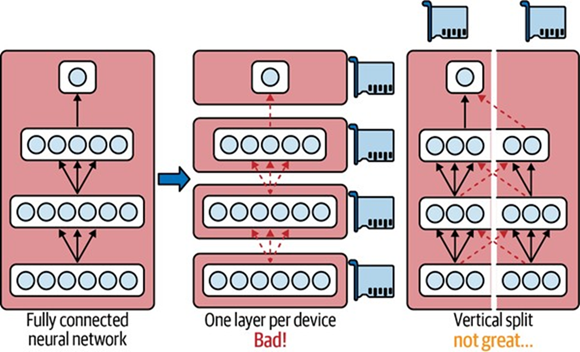
\includegraphics[width=\textwidth,height=0.65\textheight,keepaspectratio]{../machineLearningWeb/Figures/CH19/Hình_19-11.png}
            \vspace{0.2cm}
            \textit{Hình 19-11: Cắt ngang kiến trúc bằng Model Parallelism}
        \end{column}
    \end{columns}
\end{frame}

% 31
\begin{frame}{3.9 Song song Dữ liệu (Data Parallelism)}
    \begin{columns}
        \begin{column}{0.4\textwidth}
            \begin{itemize}
                \item Là cách làm phổ biến nhất.
                \item \textbf{Copy} y hệt mạng nơ-ron lên tất cả các GPU.
                \item Thay vì nạp batch size = 32 vào 1 GPU. Ta nạp 8 ảnh vào GPU 0, 8 ảnh vào GPU 1, v.v.
                \item Chúng tính toán song song Gradient, sau đó \textbf{cộng gộp Gradient lại} rồi cập nhật cho tất cả.
            \end{itemize}
        \end{column}
        \begin{column}{0.6\textwidth}
            \centering
            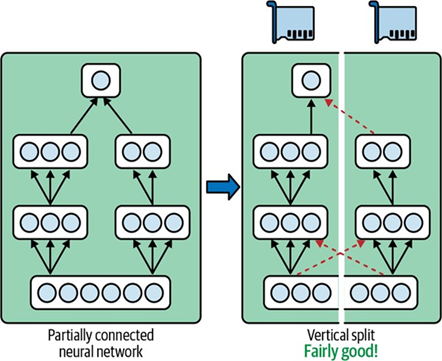
\includegraphics[width=\textwidth,height=0.65\textheight,keepaspectratio]{../machineLearningWeb/Figures/CH19/Hình_19-12.png}
            \vspace{0.2cm}
            \textit{Hình 19-12: Thuật toán Data Parallelism cơ bản}
        \end{column}
    \end{columns}
\end{frame}


%==================================================================
\section{4. Kiến trúc Đồng bộ và Bất đồng bộ}
%==================================================================

% 32
\begin{frame}{4.1 Cập nhật Đồng bộ (Synchronous Update)}
    \begin{columns}
        \begin{column}{0.4\textwidth}
            \begin{itemize}
                \item Tất cả GPU tính xong Gradient của lô ảnh của mình.
                \item Mọi người DỪNG LẠI, gửi Gradient cho nhau (Thuật toán \textbf{All-Reduce}).
                \item Trung bình cộng Gradient được tính ra, rồi tất cả cùng tiến thêm 1 bước.
                \item Điểm nghẽn: GPU nhanh phải đợi GPU chậm (Straggler).
            \end{itemize}
        \end{column}
        \begin{column}{0.6\textwidth}
            \centering
            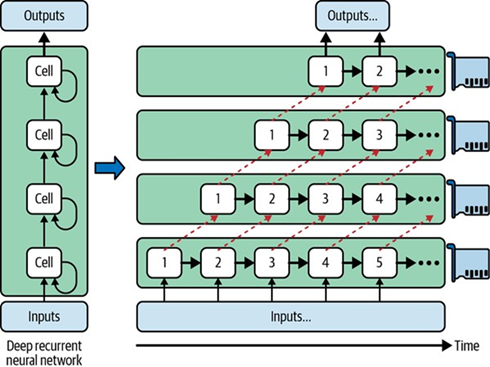
\includegraphics[width=\textwidth,height=0.65\textheight,keepaspectratio]{../machineLearningWeb/Figures/CH19/Hình_19-13.png}
            \vspace{0.2cm}
            \textit{Hình 19-13: Cập nhật Gradient Đồng bộ bằng All-Reduce}
        \end{column}
    \end{columns}
\end{frame}

% 33
\begin{frame}{4.2 Cập nhật Bất đồng bộ (Asynchronous Update)}
    \begin{columns}
        \begin{column}{0.4\textwidth}
            \begin{itemize}
                \item Có một \textbf{Parameter Server} (Máy chủ thông số) đứng giữa giữ trọng số thật.
                \item GPU 0 tính xong Gradient, quăng lên Server, Server cập nhật. GPU 0 lấy trọng số mới về làm luôn.
                \item Không ai đợi ai.
                \item Điểm trừ: Gradient bị "cũ" (Stale Gradient) khiến việc đào tạo có thể hỗn loạn (Hội tụ khó hơn).
            \end{itemize}
        \end{column}
        \begin{column}{0.6\textwidth}
            \centering
            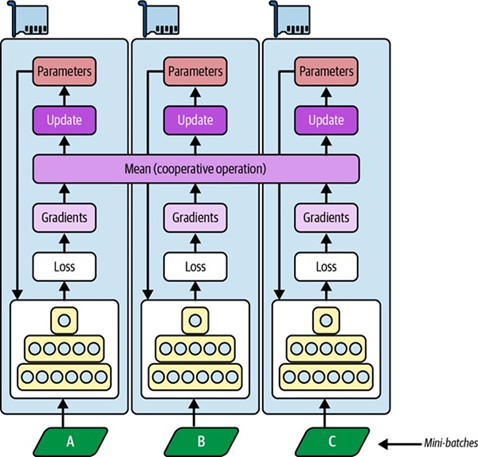
\includegraphics[width=\textwidth,height=0.65\textheight,keepaspectratio]{../machineLearningWeb/Figures/CH19/Hình_19-14.png}
            \vspace{0.2cm}
            \textit{Hình 19-14: Kiến trúc Bất đồng bộ với Parameter Server}
        \end{column}
    \end{columns}
\end{frame}


%==================================================================
\section{5. API Chiến lược Phân phối \& Huấn luyện Cụm}
%==================================================================

% 34
\begin{frame}{5.1 API \texttt{tf.distribute.Strategy}}
    \begin{itemize}
        \item Việc tự code logic chia dữ liệu và All-Reduce rất cực khổ.
        \item TensorFlow cung cấp \textbf{Distribution Strategies API}. Bạn chỉ cần viết code mô hình Keras 1 lần, TF sẽ tự lo việc phân tán nó đi đâu.
        \item Khả năng mở rộng từ 1 GPU lên cụm TPU Pods với thay đổi code tối thiểu!
    \end{itemize}
\end{frame}

% 35
\begin{frame}{5.2 MirroredStrategy (Đa GPU 1 máy tính)}
    \begin{columns}
        \begin{column}{0.45\textwidth}
            \begin{itemize}
                \item Dùng cho một máy chủ (VD: Workstation có 4 Card RTX 4090).
                \item Nó tự tạo các bản sao (Replicas) trên mỗi GPU.
                \item Sử dụng \textbf{Đồng bộ Data Parallelism} (All-Reduce qua kết nối NVLink cực nhanh).
            \end{itemize}
        \end{column}
        \begin{column}{0.55\textwidth}
            \centering
            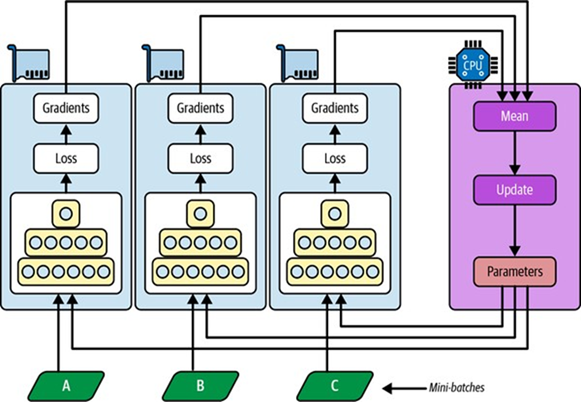
\includegraphics[width=\textwidth,height=0.65\textheight,keepaspectratio]{../machineLearningWeb/Figures/CH19/Hình_19-15.png}
            \vspace{0.2cm}
            \textit{Hình 19-15: Cơ chế của MirroredStrategy trên 1 Node}
        \end{column}
    \end{columns}
\end{frame}

% 36
\begin{frame}[fragile]{5.3 Triển khai MirroredStrategy bằng Keras}
\begin{lstlisting}[language=Python]
import tensorflow as tf

# 1. Khai bao chien luoc
strategy = tf.distribute.MirroredStrategy()

print(f"So luong thiet bi GPU: {strategy.num_replicas_in_sync}")

# 2. Xay dung va bien dich mo hinh BEN TRONG block scope
with strategy.scope():
    model = keras.models.Sequential([
        keras.layers.Dense(128, activation='relu'),
        keras.layers.Dense(10, activation='softmax')
    ])
    model.compile(loss="sparse_categorical_crossentropy", optimizer="sgd")

# 3. Huan luyen binh thuong, TF se tu chia viec!
model.fit(train_dataset, epochs=10)
\end{lstlisting}
\end{frame}

% 37
\begin{frame}{5.4 MultiWorkerMirroredStrategy (Đa máy tính)}
    \begin{columns}
        \begin{column}{0.4\textwidth}
            \begin{itemize}
                \item Khi có 5 máy tính kết nối mạng, mỗi máy có 4 GPU (Tổng 20 GPU).
                \item Thuật toán tương tự MirroredStrategy nhưng phải liên lạc All-Reduce thông qua mạng LAN/Internet (gRPC).
                \item Yêu cầu cấu hình biến môi trường \texttt{TF\_CONFIG} để các máy biết địa chỉ IP của nhau.
            \end{itemize}
        \end{column}
        \begin{column}{0.6\textwidth}
            \centering
            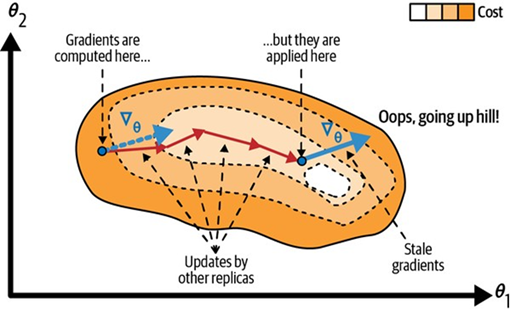
\includegraphics[width=\textwidth,height=0.65\textheight,keepaspectratio]{../machineLearningWeb/Figures/CH19/Hình_19-16.png}
            \vspace{0.2cm}
            \textit{Hình 19-16: Phân tán đào tạo trên một Cụm máy (Cluster)}
        \end{column}
    \end{columns}
\end{frame}

% 38
\begin{frame}{5.5 Huấn luyện phân tán trên Vertex AI}
    \begin{columns}
        \begin{column}{0.45\textwidth}
            \begin{itemize}
                \item Tự quản lý cụm 50 máy tính là ác mộng (Lỗi ổ cứng, sập mạng, quá nhiệt).
                \item Đẩy code lên \textbf{Vertex AI Custom Training}.
                \item Google sẽ khởi động 50 cái máy (Compute Engine) kết nối sẵn, cài sẵn TF, chạy code của bạn. Chạy xong tự động tắt máy.
            \end{itemize}
        \end{column}
        \begin{column}{0.55\textwidth}
            \centering
            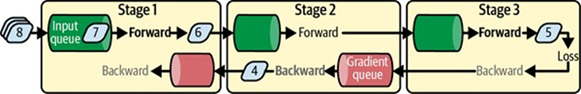
\includegraphics[width=\textwidth,height=0.6\textheight,keepaspectratio]{../machineLearningWeb/Figures/CH19/Hình_19-17.png}
            \vspace{0.2cm}
            \textit{Hình 19-17: Đóng gói Code bằng Docker để đưa lên Cloud}
        \end{column}
    \end{columns}
\end{frame}

% 39
\begin{frame}{5.6 Điều chỉnh Siêu tham số (Hyperparameter Tuning)}
    \begin{columns}
        \begin{column}{0.4\textwidth}
            \begin{itemize}
                \item Làm sao để biết Learning Rate = $0.01$ hay $0.001$ là tốt nhất? Batch Size = 32 hay 64?
                \item Vertex AI cung cấp dịch vụ Vizier. Thuật toán Tối ưu hóa Bayesian sẽ đoán thử các cặp thông số và chạy thử nghiệm (Trial).
                \item Giúp tìm ra kiến trúc tốt nhất mà không cần thử tay mù quáng.
            \end{itemize}
        \end{column}
        \begin{column}{0.6\textwidth}
            \centering
            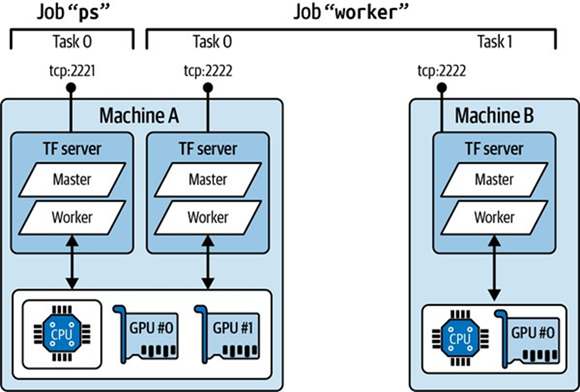
\includegraphics[width=\textwidth,height=0.65\textheight,keepaspectratio]{../machineLearningWeb/Figures/CH19/Hình_19-18.png}
            \vspace{0.2cm}
            \textit{Hình 19-18: Quá trình tìm kiếm siêu tham số qua các Trial}
        \end{column}
    \end{columns}
\end{frame}


%==================================================================
\section{6. Tổng kết}
%==================================================================

% 40
\begin{frame}{Tổng Kết Chương 19}
    \begin{itemize}
        \item Để đưa AI phục vụ hàng triệu người dùng, ta dùng \textbf{TF Serving}.
        \item Đưa AI xuống điện thoại/web để có độ trễ siêu thấp bằng \textbf{TFLite} \& \textbf{TF.js}.
        \item Gia tốc huấn luyện với \textbf{GPU / TPU} giúp giảm thời gian từ hàng năm xuống còn vài ngày.
        \item API \textbf{Distribution Strategies} giúp code linh hoạt mở rộng từ 1 máy lên quy mô Cluster đám mây.
        \item Hệ sinh thái TensorFlow cung cấp bộ công cụ E2E (End-to-End) hoàn hảo cho mọi quy mô doanh nghiệp.
    \end{itemize}
\end{frame}

% 41
\begin{frame}
    \centering
    \Huge \textbf{HỎI \& ĐÁP}
\end{frame}

\end{document}
